\documentclass{beamer}
\usepackage[utf8]{inputenc}
\usepackage{datetime2}
\usepackage{multicol}
\usepackage{tikz}
\usepackage{calc}
\usepackage{csquotes}
\usepackage[ngerman]{babel}
\usetheme{metropolis}
\usepackage[
style=alphabetic,
citestyle=authoryear,
sorting=nyt]{biblatex}
\addbibresource{literatur.bib}
% % Definition Progressbar
\makeatletter
\newlength{\custom@progressinheadfoot}
\setbeamertemplate{progress bar in head/foot}{
	\nointerlineskip
	\setlength{\custom@progressinheadfoot}{%
		\paperwidth * \ratio{\insertframenumber pt}{\inserttotalframenumber pt}%
	}%
	\begin{beamercolorbox}[wd=\paperwidth]{progress bar in head/foot}
		\begin{tikzpicture}
		\draw[bg, fill=bg] (0,0) rectangle (\paperwidth, 0.17em);
		\draw[fg, fill=fg] (0,0) rectangle (\custom@progressinheadfoot, 0.17em);
		\end{tikzpicture}%
	\end{beamercolorbox}
}
\addtobeamertemplate{footline}{}{%
	\usebeamertemplate*{progress bar in head/foot}%
}
\title{Softwarearchitekturen}
\subtitle{Wie wird ein Entwurf für eine Softwarearchitektur erzeugt?}
\author{Sidney Kuyateh \& Steffen Walter}
\institute{Duale Hochschule Baden-Württemberg}
\date{\today}
\setbeamercolor{progress bar in head/foot}{fg=orange, bg=lightgray}
\begin{document}
	\maketitle
	\begin{frame}[allowframebreaks]{Überblick}
			\tableofcontents[sectionstyle=show, subsectionstyle=show/shaded,]
	\end{frame}
	%%%% Steffen %%%%
		\section{Einführung}
		\metroset{block=fill}
		\subsection{Einführung Softwarearchitekturen}
		\begin{frame}{Einführung Softwarearchitekturen}
			\begin{block}{Definition 1:}
				\enquote{Softwarearchitektur: [...] Strukturierte oder hierarchische Anordnung der Systemkomponenten sowie Beschreibung ihrer Beziehungen.} (\cite{balzert} Seite 520)
			\end{block}
			\begin{block}{Definition 2:}
				\enquote{Strukturen eines Softwaresystems: Softwareteile, die Beziehungen zwischen diesen und die Eigenschaften der Softwareteile und ihrer Beziehungen.} (\cite{clements})
			\end{block}
		\end{frame}
		\section{Architektursichten}
		\subsection{Perspektiven}
			\begin{frame}{Perspektiven}
				\begin{columns}
				\column{0.5\textwidth}
				\begin{itemize}
					\item Es existiert kein Modell, welches alle relevanten Informationen beinhaltet
					\item 4+1-Sichtenmodell (vgl. \cite{4+1})
						\begin{itemize}
						\item Logische Sicht
						\item Prozessorientierte Sicht
						\item Entiwicklungsorientierte Sicht
						\item Physische Sicht 
						\end{itemize} 
				\end{itemize}
			   	\column{0.5\textwidth}
			   	\begin{figure}
					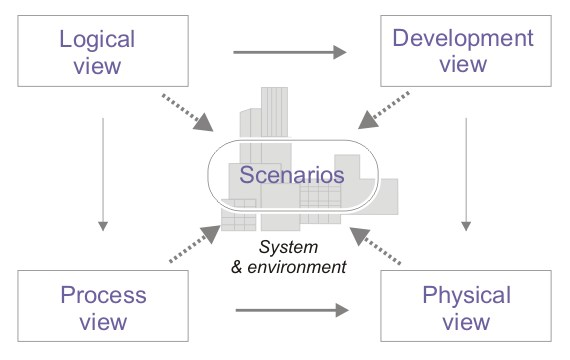
\includegraphics[width=\textwidth]{4+1.jpg}
					\caption{Darstellung 4+1-Sichtenmodell (vgl. \cite{4+1pic})}
				\end{figure}
			\end{columns}
			\end{frame}
			\subsection{Notationen}
			\begin{frame}{Notationen}
		
			\end{frame}
		
		\section{Architekturmuster}
			\subsection{Schichtenarchitektur}
			\begin{frame}{Schichtenarchitektur}
			
			\end{frame}
			\subsection{Repository-Architektur}
			\begin{frame}{Repository-Architektur}
			
			\end{frame}	
			\subsection{Client-Server-Architektur}
			\begin{frame}{Client-Server-Architektur}
			
			\end{frame}
			\subsection{Pipes-and-Filter-Architektur}
			\begin{frame}{Pipes-and-Filter-Architektur}
			
			\end{frame}	
	%%%% Sidney %%%%
	\section{Softwarearchitektur}
		\subsection{Definition des Begriffs Softwarearchitektur}
			\begin{frame}{Definition des Begriffs Softwarearchitektur}
				\begin{itemize}
					\item Grundlegende Organisation eines Systems (vgl. \cite{gi-lexikon})
					\item Bestehend aus folgenden Elementen:
					\begin{itemize}
						\item Komponenten
						\item Beziehungen zwischen den Komponenten
						\item Beziehungen zur Umgebung
						\item Prinzipien, die Entwurf und Evolution des Systems beschreiben
					\end{itemize}
				\end{itemize}
			\end{frame}
		\subsection{Weiterer Test}
			\begin{frame}{Weiterer Test}
				bla bla blub
			\end{frame}
	\begin{frame}[allowframebreaks]
		\frametitle{Quellen}
		\printbibliography[heading=none]
	\end{frame}
\end{document}


